\section{Architecture of the application}\label{design}
The architecture of the application is split into two parts, the UI a user sees and interacts with, and the underlying functionality, commonly referred to as the frontend and backend respectively. In this section I will describe considerations and decisions made regarding both, starting with the frontend.

\subsection{Responsive and dynamic pages}

Modern websites are generally expected to be usable on many different kinds of devices while having a consistent UI across varying screen sizes, in order to meet this expectation the responsiveness is a key part of designing the HTML templates \cite{responsive_article}.\\
\begin{figure}[b!]
\centering
\hrule
\vspace*{0.2cm}
\begin{minipage}{.5\textwidth}
\centering
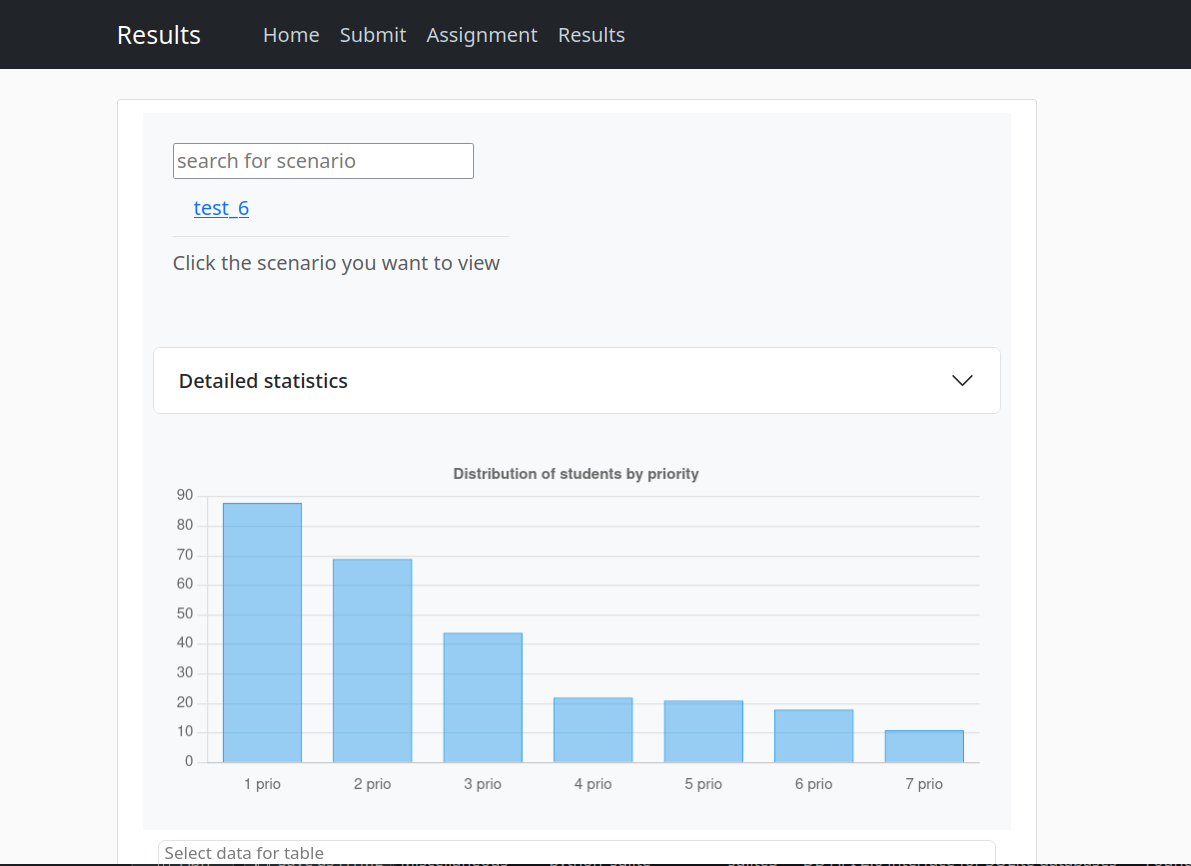
\includegraphics[width=\textwidth]{results_big}
\caption{The results page of the application in its default view.}
\label{fig:design_res_big}
\end{minipage}%
\hspace{1cm}
\begin{minipage}{.4\textwidth}
\centering
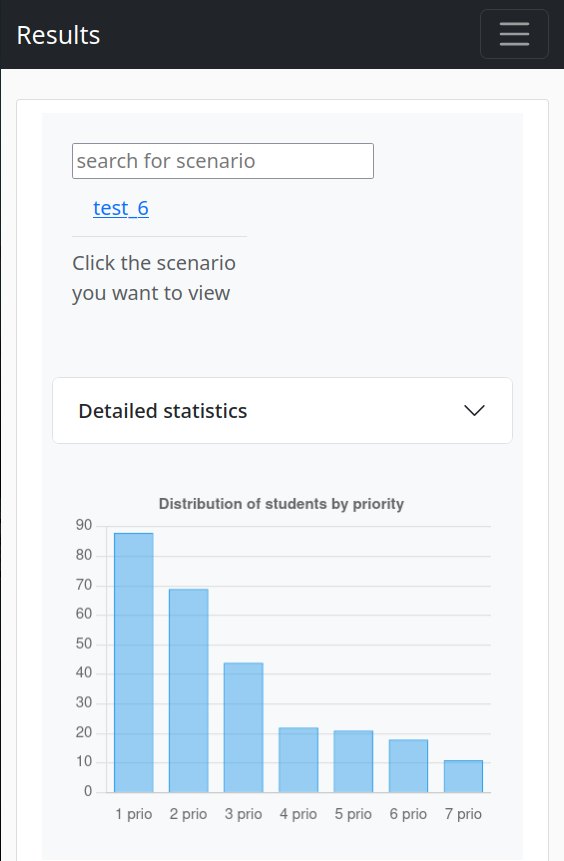
\includegraphics[scale=.3]{results_small}
\caption{The results page of the application in a narrow view. The navigation bar at the top, has been collapsed into a ``hamburger menu''.}
\label{fig:design_res_small}
\end{minipage}
% \hrule
\end{figure}
To help in the development of the templates I use the  CSS framework Bootstrap, which includes many predefined components which can be used in the design of the UI. Bootstrap components are designed with responsiveness in mind, it allows a developer to use a component which will render differently depending on screen size, like the navigation bar at the top of the page illustrated in Figure \ref{fig:design_res_big} and \ref{fig:design_res_small}.\\This use of predefined responsive components instead of explicitly defining what small, medium and large screens are and designing a page for each, reduces the complexity of designing a modern web UI.
\\\\
\begin{figure}[t!]
\centering
	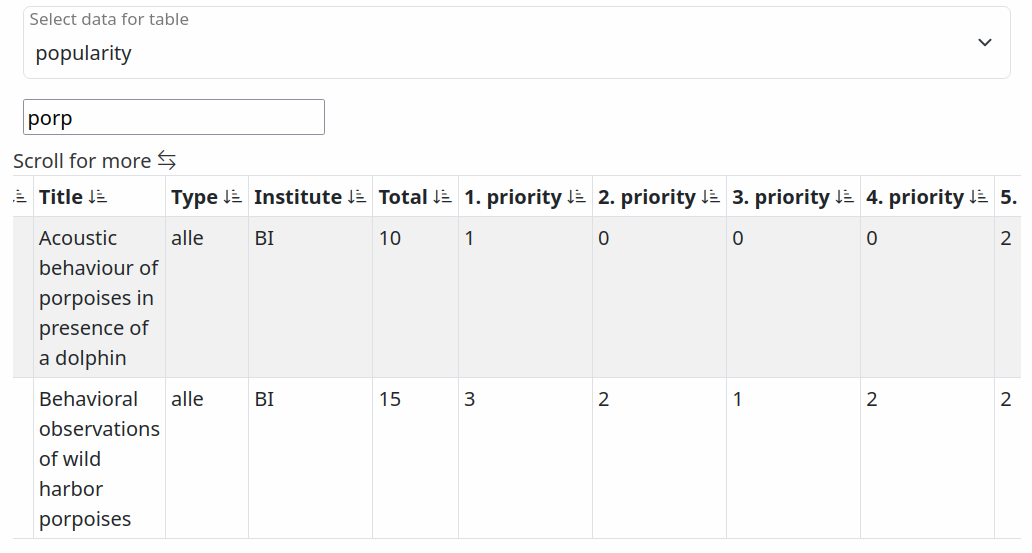
\includegraphics[width=.8\textwidth]{search_sort_table.png}
	\caption{An example of a table which is too wide to be shown in its entirety and where a user has used the search field to limit the displayed entries to those containing the string ``porp''.}
	\label{fig:table_search_sort}
	\hrule
\end{figure}
The Django template language supports the inclusion of one template in another and the creation of blocks\footnote{Also supported by other template languages, e.g. Jinja2.}, these features in combination means a single file can define the UI across multiple pages.\\This approach ensures a consistent UI without repeating code, and if the design needs to be changed the change can be made in a single file instead of changing the same thing in all the templates.
\\\\
In addition to having responsive pages I also wanted the pages to be somewhat dynamic, meaning some elements on the page would react or change in response to the user interaction without re-rendering the entire template. Bootstrap does include some dynamic components, like an accordion in which advanced options can be hidden, but more advanced features would have to be build using some form of JavaScript. I decided to include the JavaScript framework VueJS in my templates, which allowed me to build small components with the necessary functions and data, and then attach these components to elements defined in my HTML templates.\\\\
The combination of VueJS, Django Templating language and bootstrap allows me to build, among other things, tables which will be populated with data chosen from a drop-down menu, that are sortable and searchable on all fields and if the table is populated with too much data to fit the screen on which it is shown, the user can scroll sideways to view the rest of the data, example shown in Figure \ref{fig:table_search_sort}.
\begin{figure}[H]
\centering
% \hrule
%\vspace*{0.2cm}
%\begin{minipage}{.4\textwidth}
\centering
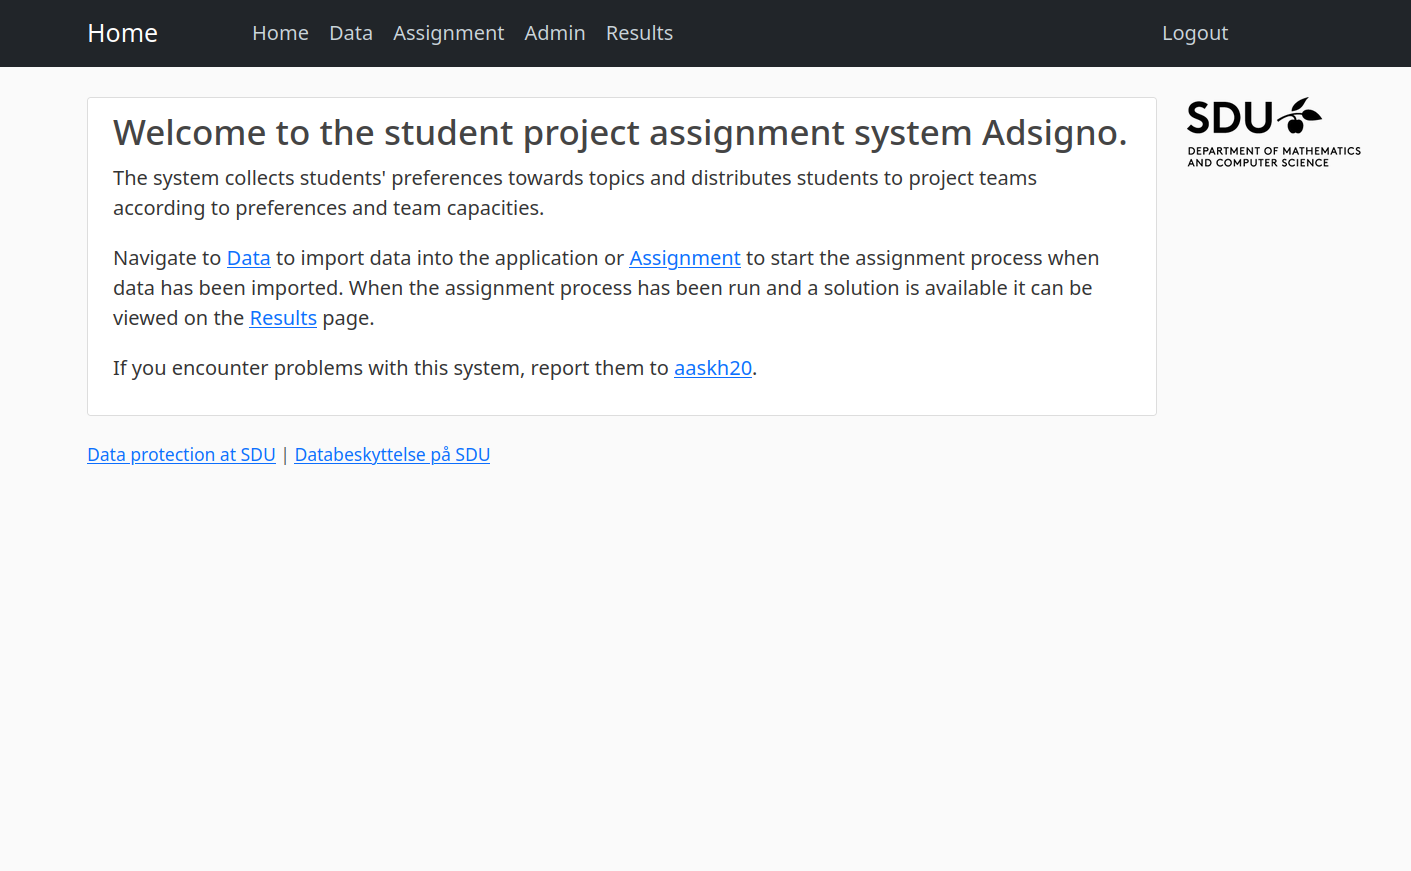
\includegraphics[width=.7\textwidth]{live_page/home}
\caption{Home page}
\label{fig:design_home}
\vspace*{0.1cm}
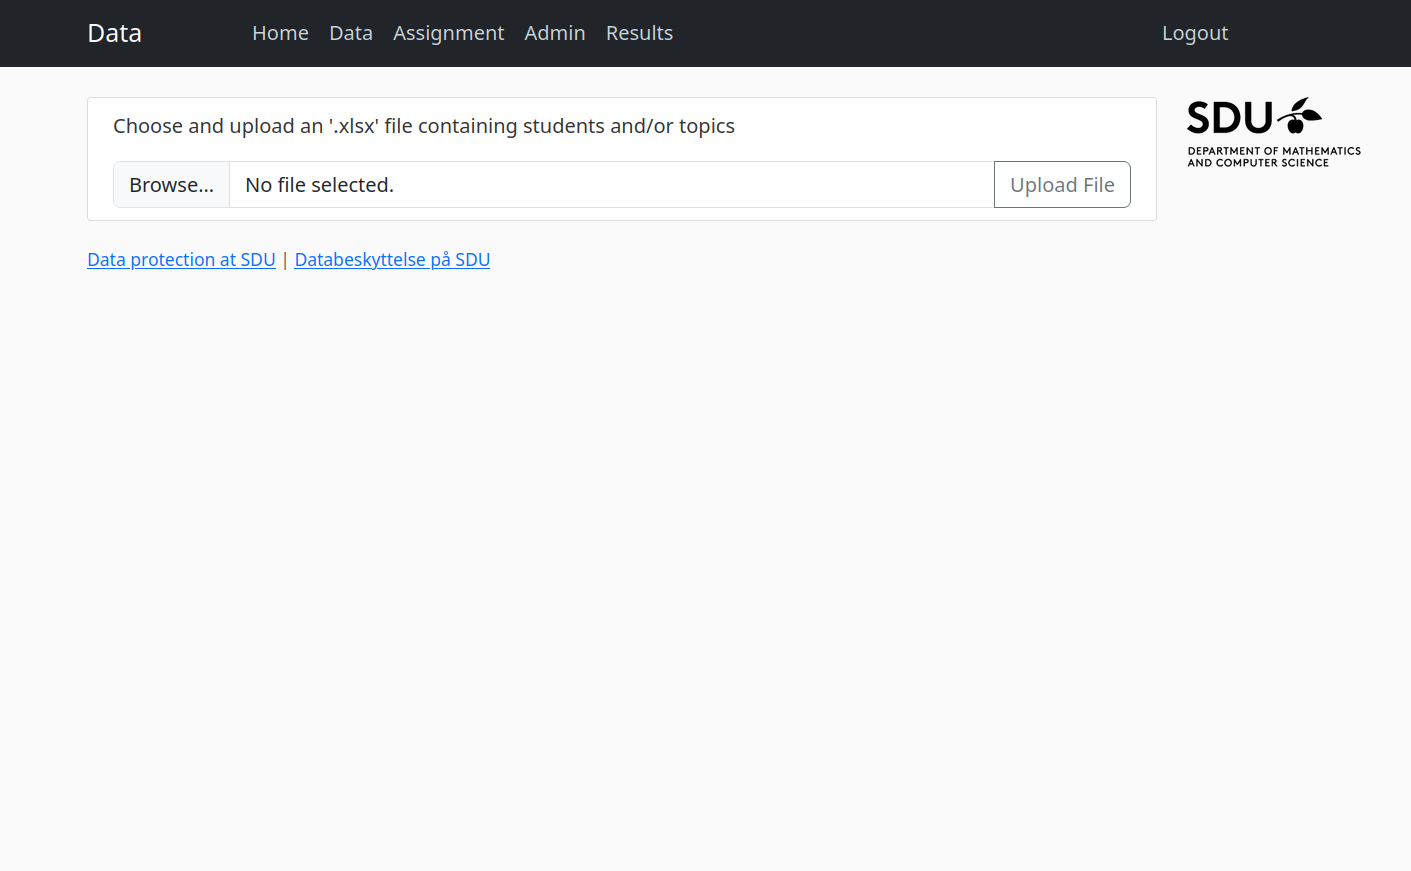
\includegraphics[width=.7\textwidth]{live_page/upload}
\caption{Data page}
\label{fig:design_data}
\vspace*{0.1cm}
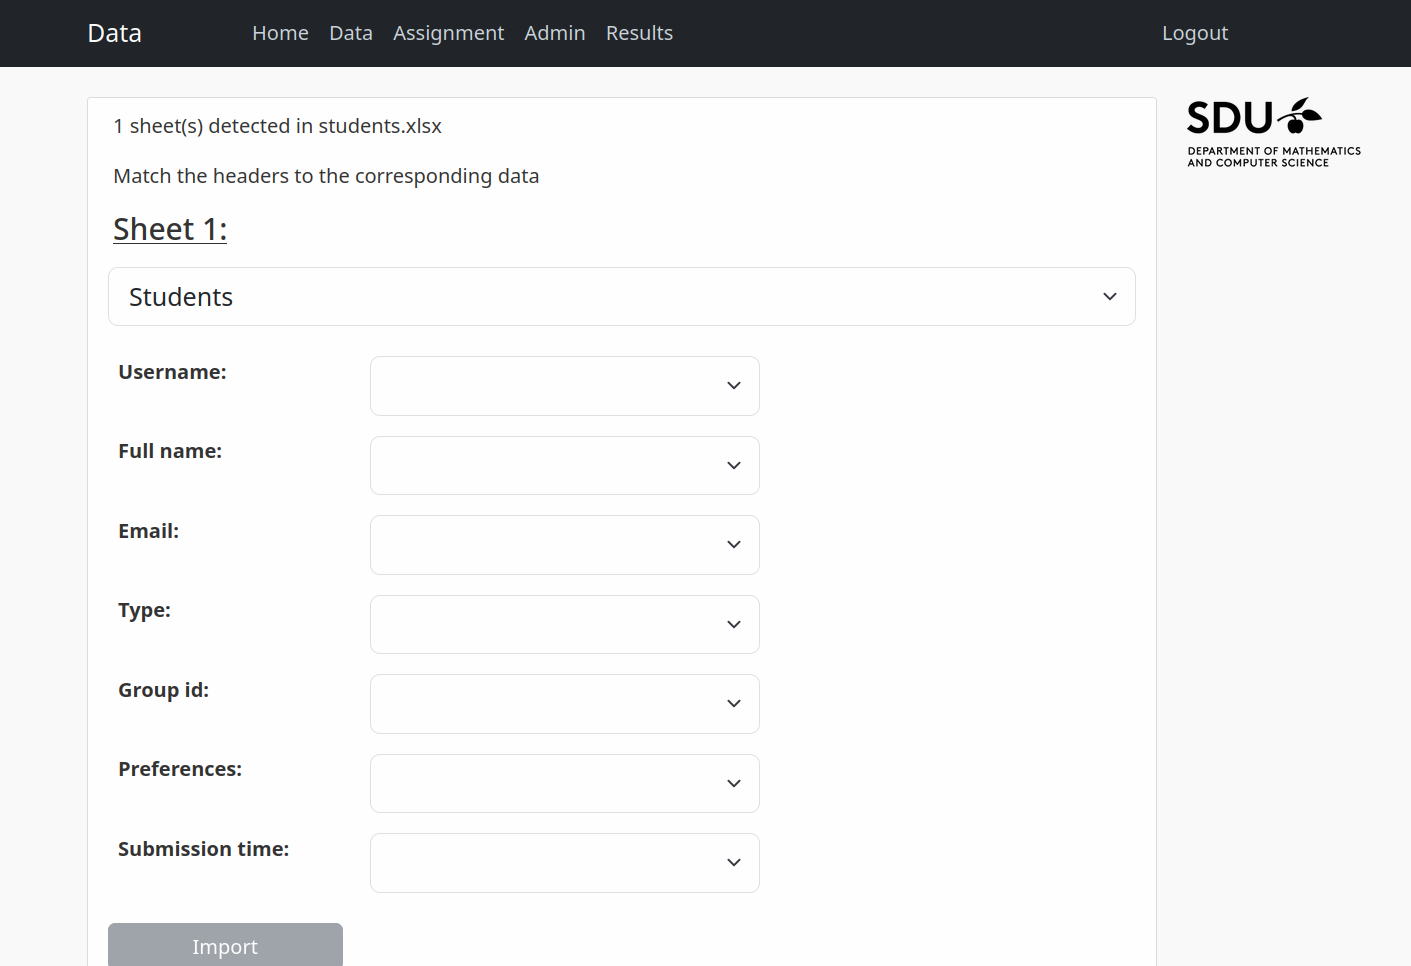
\includegraphics[width=.7\textwidth]{live_page/assign}
\caption{Header/data matching page}
\label{fig:design_ass}
\end{figure}
%\end{figure}
%\end{minipage}%
%\hspace{1cm}
%\begin{minipage}{.4\textwidth}

\subsection{Workflow}
When designing the web site, I wanted to match the workflow shown in Figure \ref{fig:intro_old} as close as possible, with a page for each part aiming for a user experience as intuitive and familiar to the users as possible. This approach resulted in four distinct pages: home, data, assignment and results. All pages have the same navigation bar at the top allowing for easy navigation between them, and an additional page for administrators to assign permissions and make changes to the stored data. 
\\\\
The home page, shown in Figure \ref{fig:design_home}, is the first thing a user sees,  it serves as a welcome page and contains a short description of the application.
\\\\
The data page, Figure \ref{fig:design_data}, is where new topics and students are imported into the application. Excel spreadsheets containing students and/or topics, examples of these files are illustrated in Figures \ref{fig:design_studs} and \ref{fig:design_tops}, can be uploaded and the user is then transferred to a page on which the headers of the uploaded document must be matched with the required data, Figure \ref{fig:design_ass}. This approach means the formatting of the file is less strict, while ensuring the data is imported correctly. The matching could be done automatically based on the title of the headers, this approach was however shown to be more robust during testing.%\\\\
\begin{figure}[b!]
\hrule
\vspace*{0.2cm}
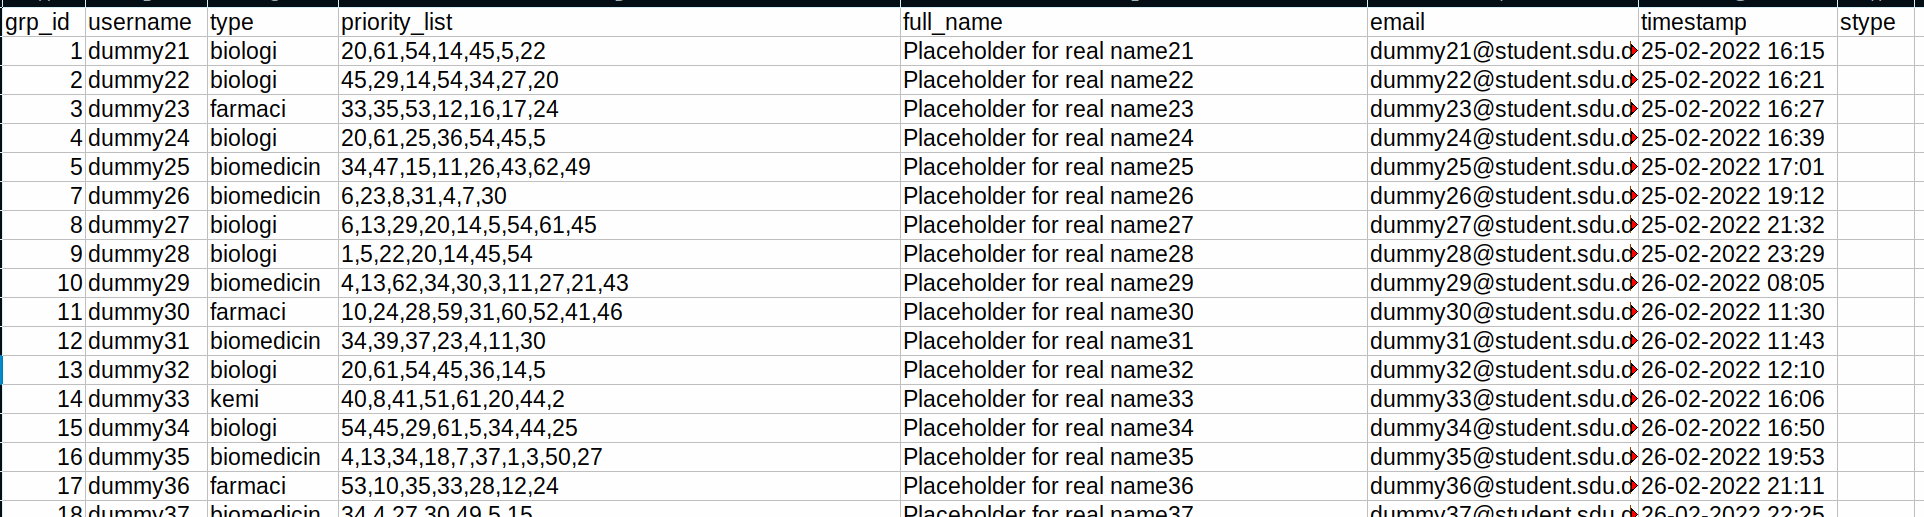
\includegraphics[width=.9\textwidth]{docs/students}
\caption{An example of a file containing information about the students involved in a case.}
\label{fig:design_studs}
\vspace*{0.1cm}
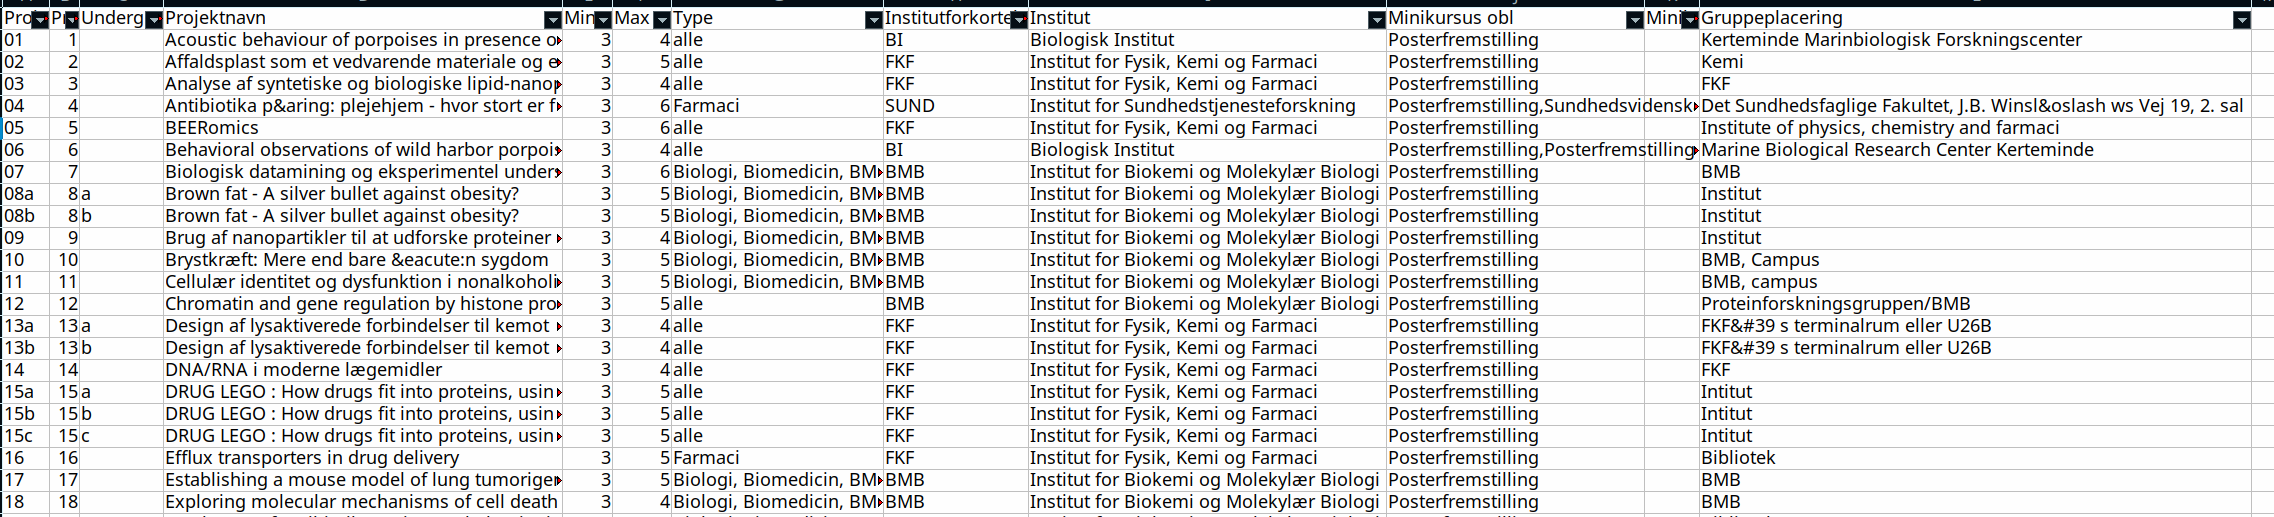
\includegraphics[width=.9\textwidth]{docs/topics}
\caption{An example of a file containing information about the topics to which students should be assigned.}
\label{fig:design_tops}
\end{figure}
\\\\
When a case, consisting of both students and topics, has been imported into the application, the allocation process can be started from the assignment page shown in Figures \ref{fig:design_compute} and \ref{fig:design_compute_adv}. All the parameters for the process are presented and adjustable on this page.
\\\\
On the results page the different scenarios are listed at the top, along with a search field to quickly find a specific scenario. Selecting a scenario will present the details of the scenario beginning with a bar chart, pictured in Figure \ref{fig:design_res_big} showing the distribution of students according to their priorities, followed by the table shown in Figure \ref{fig:table_search_sort} containing detailed information chosen from a drop-down menu.
\\\\
In order to assign permissions to users and view/update the data in the database, authorized users have access to the Django administration page, Figure \ref{fig:design_admin}, on which these actions can be performed. 
\begin{figure}[H]
\centering
\vspace{-2cm}
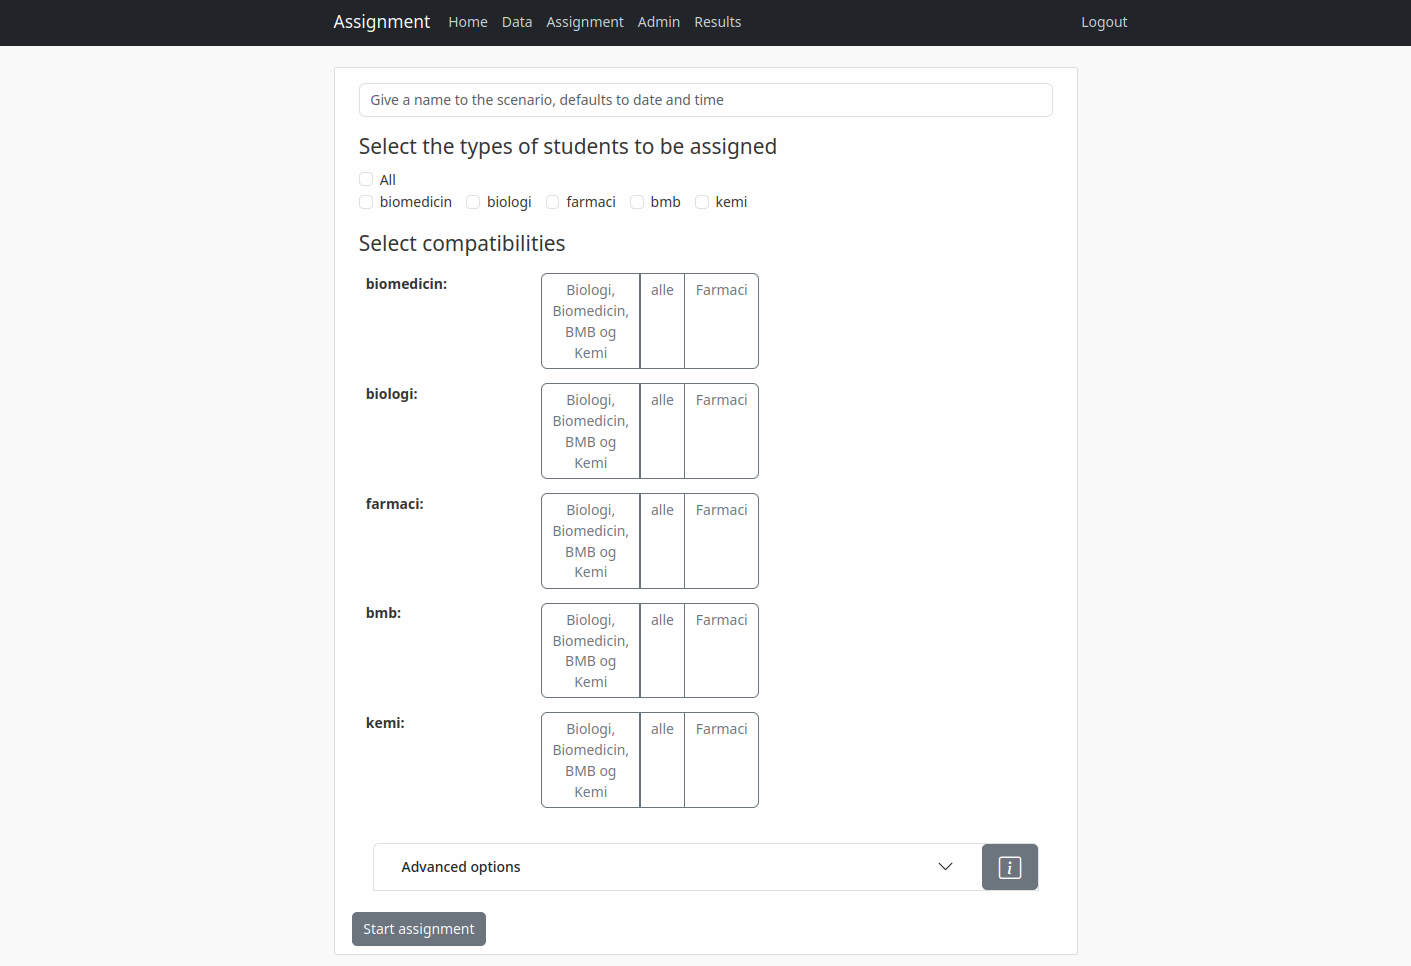
\includegraphics[width=.7\textwidth]{live_page/compute}
\caption{Assignment page, basic view}
\label{fig:design_compute}
\vspace*{0.1cm}
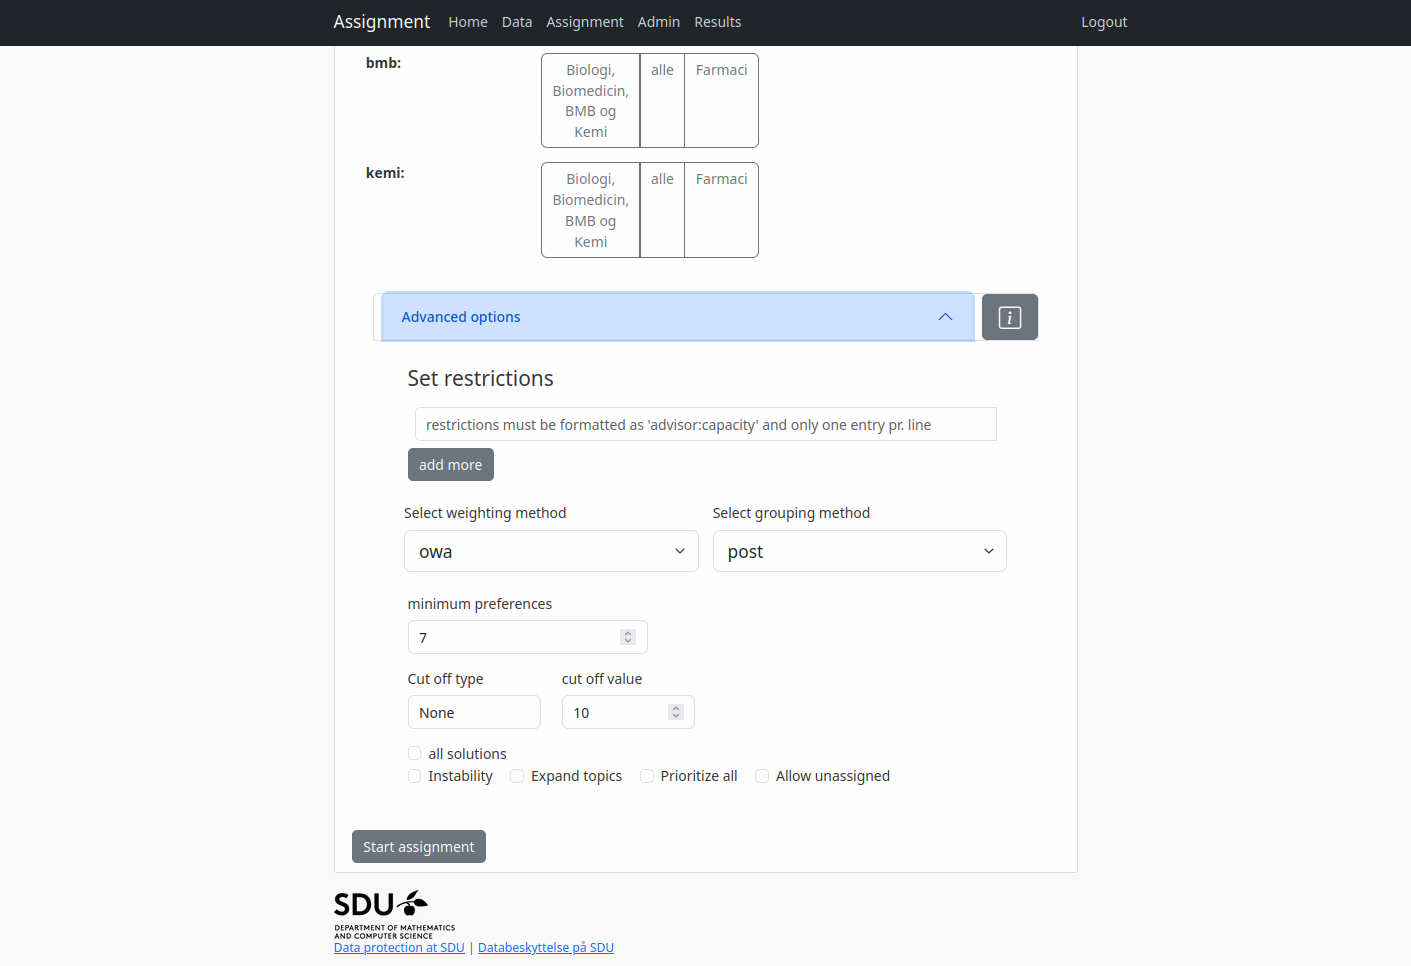
\includegraphics[width=.7\textwidth]{live_page/compute_adv}
\caption{Assignment page, showing advanced options}
\label{fig:design_compute_adv}
\vspace*{0.1cm}
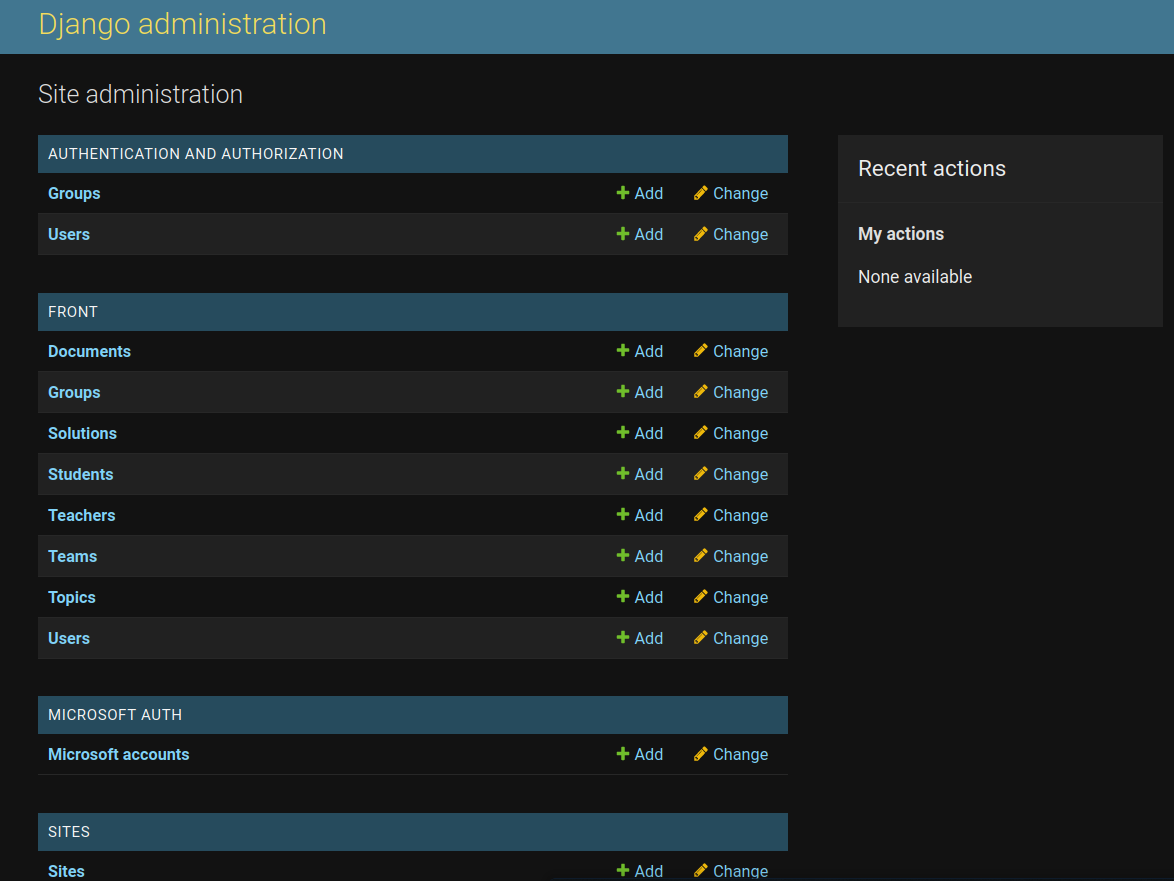
\includegraphics[width=.7\textwidth]{live_page/admin}
\caption{Administration page}
\label{fig:design_admin}
%\end{minipage}
%\caption*{A collection of screenshots showing the pages of the application, with the exception of the results page which is pictured in Figure \ref{fig:design_res_big} and \ref{fig:table_search_sort}.}
%\vspace*{0.2cm}
%\hrule
\end{figure}
\subsection{Database}
Since the database supporting the application is an SQLite instance very little configuration is needed before it can be used. When building a Django application and using an SQLite database the only configuration strictly needed is done by default and consists of two lines of code. The first line defines the engine needed to communicate with the database and the second line is a path to the file containing the database.
\\
\begin{figure}[t]
\centering
% \hrule
% \vspace*{0.2cm}
\begin{minted}{python}
from django.db.backends.signals import connection_created

def activate_wal_mode(sender, connection, **kwargs):
    """Enable Write ahead logging in sqlite."""
    if connection.vendor == 'sqlite':
        cursor = connection.cursor()
        cursor.execute('PRAGMA journal_mode=WAL;')

connection_created.connect(activate_wal_mode)
\end{minted}
\caption{Code snippet enabling WAL-mode on the SQLite database during initialisation}
\label{des:code_wal}
\hrule 
\end{figure}
To addres the concerns regarding concurrency however, means a little more configuration is needed. The ``timeout'' value is increased to 20 this allows a thread wanting to access the database to wait for up to 20 seconds in case the database is currently locked by another thread.
\\
Another attempt at mitigating potential problems arising from concurrent access to the database is to enable Write Ahead Logging mode (WAL-mode). This is done by including the code from Figure \ref{des:code_wal} in the \verb|/front/__init__.py| file, which means it will be executed when the application is initialised.\\
By default an instance of an SQLite database will write changes directly to the database file, while saving a separate rollback journal. WAL-mode instead appends any changes to the end of a buffer file without changing the contents of the database file, these changes are written to the database file when the wal buffer reaches 1000 pages by default.\\
When a read operation is started a mark is set at the current end of the WAL buffer, this mark will not change during the read. The reader then reads from the beginning of the WAl buffer to the marked end of the buffer and, if the needed data was not found, it continues its operation in the original database file.\\
This approach means a write operation can be performed without interfering with an ongoing read operation, write operations can however only be performed by one thread at a time.

\subsubsection{Tables and relations}
\begin{figure}[t!]
\centering
\vspace{-2cm}
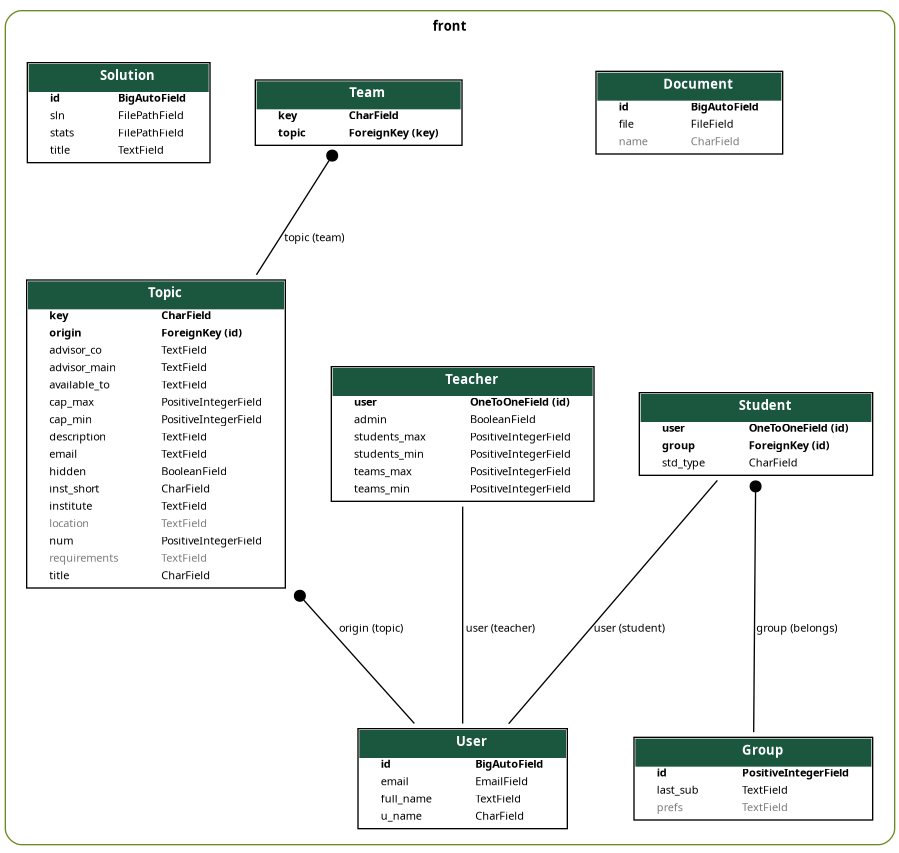
\includegraphics[width=.8\textwidth]{appendix/erd.png}
\caption{ER diagram of the database used in the application. Automatically generated with "django-extensions" and Graphviz. }
\label{fig:er_dia}
\hrule
\end{figure}
All tables and relations used in  connection with the application are defined in the \verb|/front/models.py| file. When designing the database I started by making the tables ``Topic'' and ``Student'' since these were the entities that needed to be paired, building from this starting point the database evolved into what is shown in Figure \ref{fig:er_dia}. While the actual pairing is between a group of students, consisting of one or more students and a project, this relation is not explicitly present in the Entity Relation (ER) diagram or the database but rather contained in the Solution entity as the ``sln'' attribute. The Solution entity contains as attributes paths to the files created by the allocation application, and a title for users to easily differentiate between the solutions when they are listed on the results page.
\\\\
While importing documents containing multiple students and/or topics are done on the data page, if a user wants to create, read, update or delete\footnote{Commonly referred to as CRUD operations} individual entries in the database, the default admin page created when starting a new django project is utilised. On this page any user who is signed in and has the proper permissions can edit or create individual entries in the database and delete one or more entries.
\subsection{User authentication}\label{sec:login}
Some of the pages in the web application contain information which should not be publicly accessible, like the email and user name of the students being assigned to topics, and functions that only authorised users should have access to, like starting the allocation process.\\
In order to restrict access to these pages to authorized users, a login system has been implemented where users can login using their SDU accounts.\\
When a user logs in with their SDU credentials, their account will either be linked to an existing authentication user with the same email address or a new user will be created and then linked to the SDU account.\\\\
When the application is started a super user with access and permissions to do everything is created, with credentials specified in a \verb|.env| file, this file will be described on page  \pageref{sec:cont}. The email specified for this user determines which SDU user is able to set permissions for all subsequent users.\\
Five permission levels exist, each building on top of the previous one:
\begin{enumerate}
\item A guest is someone who is not logged in and only has access to the welcome page and the option to login.
\item A logged in user is allowed to view the solution of an assignment.
\item Teachers are allowed to upload documents to the system.
\item Users designated as ``staff'' are allowed to start the assignment process and view the admin page but, by default not view or edit any data in the database.
\item Super users who are allowed to make changes on the admin page.
\end{enumerate}
Super users have the ability to assign permissions to staff users, allowing them to view and/or edit specific tables in the database.\\\\
I made the decision to rely on SDU authentication for user authentication, because the application aims to solve a problem experienced at SDU.\\
The problem might not however be exclusive to SDU but since the authentication at SDU is done using Azure Active Directory(AAD), it is however fairly simple to migrate the application to any other organization or entity who relies on AAD for user authentication, by creating an app registration in AAD and entering three codes into the \verb|.env| file.